\section{Git Concepts}
\label{sec:concepts}

Git is distributed version control system.  It's ``distributed" because a complete copy of the version history resides on your computer and every other contributors' computer in a hidden directory.  This means you can work on your paper online or offline and Git is really fast.

I'm going to walk you though using Git with the command line.  You will probably decide to use a GUI client (link in section \ref{gitpackages}), but if you understand the concepts of what is going on, using the GUI tool will be much easier.

I have a directory called ``myproject" that is empty, I want to write a paper here and use Git for version control.  First I need to initiate the repository:

\begin{quote}
	\begin{verbatim}
		> git init
	\end{verbatim}
	Initialized empty Git repository in /Users/tazz/myproject/.git/
\end{quote}

Great, now I can work on my file just like I normally would.  I'm creating a basic LaTeX document for another handout.  I've created the initial version and I want to commit it to the repository.

\begin{quote}
	\begin{verbatim}
		> git add basic.tex
	\end{verbatim}
\end{quote}

The changes (which in this case is the entire file) of basic.tex are now ``staged".  The staging area is where you select which set of changes you want to group together as a single commit.  If I type:

\begin{quote}
	\begin{verbatim}
		> git status
	\end{verbatim}
\end{quote}

I get the following information:

\begin{quote}
	\begin{verbatim}
# On branch master
#
# Initial commit
#
# Changes to be committed:
#   (use "git rm --cached <file>..." to unstage)
#
#	new file:   basic.tex
#

\end{verbatim}
\end{quote}

Ok, but I have some other work I want to do before I commit.  I need to create a readme file in the same directory.  I've created the file, so I'm now going to stage it as well.

\begin{quote}
	\begin{verbatim}
		> git add README.md
	\end{verbatim}
\end{quote}

I should also note that if you want to stage all changes in a directory you can type the following:

\begin{quote}
	\begin{verbatim}
		> git add .
	\end{verbatim}
\end{quote}

Ok, now I'm ready to commit:

\begin{quote}
	\begin{verbatim}
		> git commit -m "Initial version of LaTeX document and Readme"
	\end{verbatim}
\end{quote}

Git returns:

\begin{quote}
	\begin{verbatim}
[master (root-commit) 1c583ce] Initial version of LaTeX document and Readme
 2 files changed, 13 insertions(+)
 create mode 100644 README.md
 create mode 100644 basic.tex
	\end{verbatim}
\end{quote}

Now, what's really great about this is that now all of that work I did is safe.  I can delete both of those files in my working directory and I'd still be able to retrieve them.

So, the basic concept is that you work on files in your working directory, stage the changes and finally commit those changes to the repository.  Visually, it might look like figure \ref{fig:diagram}:

\begin{figure}[h]
	\centering
  	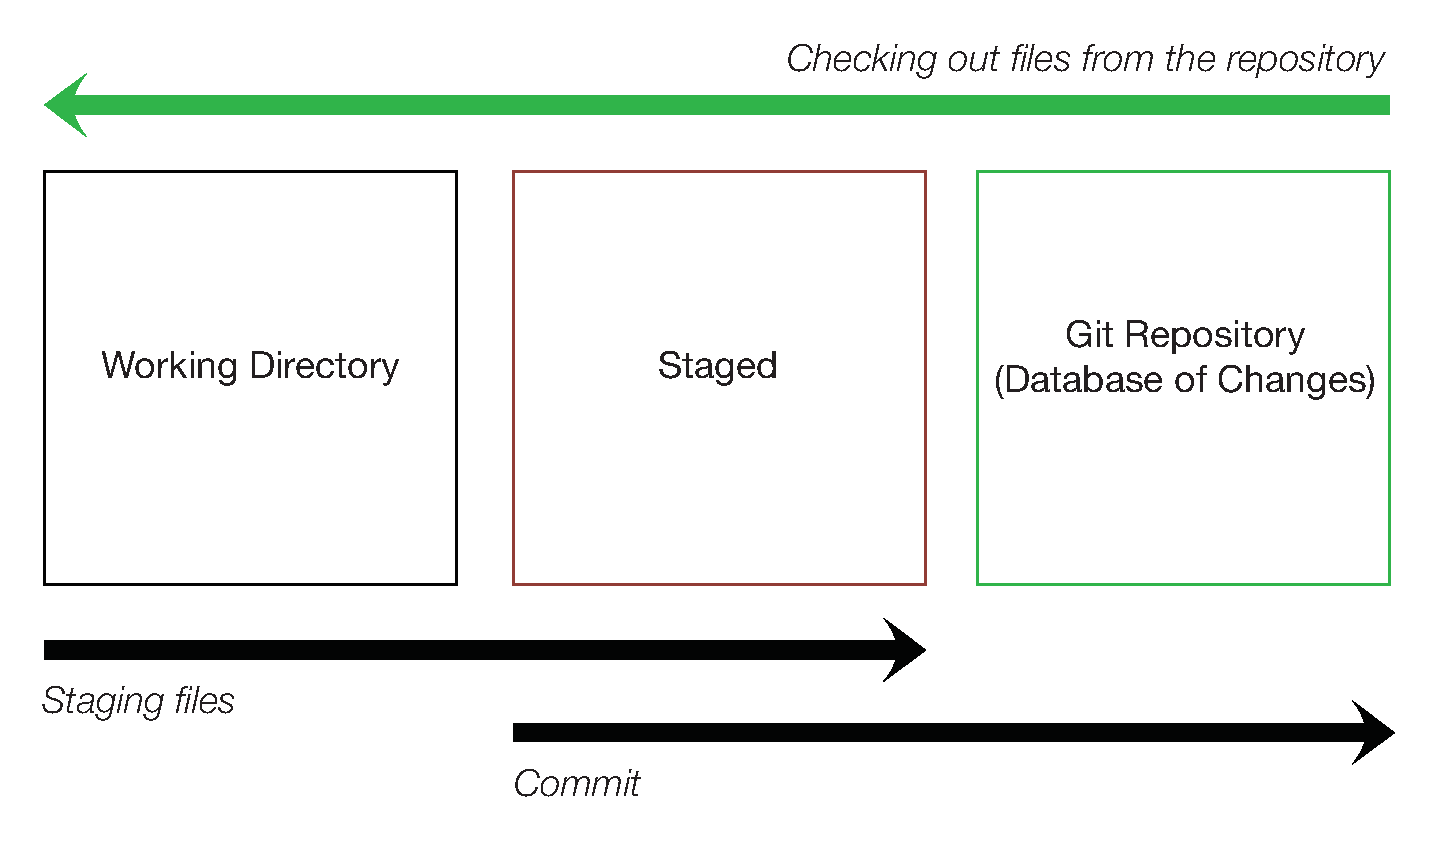
\includegraphics[width=6in]{graphics/diagram.eps}
  	\caption{You first stage a set of files, then once you are done, you commit}
  	\label{fig:diagram}
\end{figure}

Suppose I've made a change to ``basic.tex" I want to commit.

\begin{quote}
	\begin{verbatim}
		> git add basic.tex
		> git commit -m "Added fullpage to basic.tex document"
	\end{verbatim}
\end{quote}

Git returns:

\begin{quote}
	\begin{verbatim}
		[master dd367b7] Added fullpage to basic.tex document
 1 file changed, 1 insertion(+)
	\end{verbatim}
\end{quote}

You can see the history of commits by typing:

\begin{quote}
	\begin{verbatim}
		> git log
	\end{verbatim}
\end{quote}

Git returns:

\begin{quote}
	\begin{verbatim}
		commit dd367b7cfd99c3a865d2e655938a8fa8c5e72fd6
Author: Ben Smith 
Date:   Mon Oct 1 14:27:40 2012 -0700

    Added fullpage to basic.tex document

commit 1c583cecf971e0ef0bc155ed153275c3307e365e
Author: Ben Smith 
Date:   Mon Oct 1 14:21:34 2012 -0700

    Initial version of LaTeX document and Readme
	\end{verbatim}
\end{quote}

You can also generate a ``diff" file, a file containing the changes between two different versions, by typing (on one line):

\begin{quote}
	\begin{verbatim}
		> git diff 
	dd367b7cfd99c3a865d2e655938a8fa8c5e72fd6..1c583cecf971e0ef0bc155ed153275c3307e365e
 > ~/desktop/diff.diff
	\end{verbatim}
\end{quote}

Where ``dd367b7cfd99c3a865d2e655938a8fa8c5e72fd6" and ``1c583cecf971e0ef0bc155ed153275c3307e365e" are the two commit identifiers.  You can also use ``HEAD" to specify the latest version.